% Exposé V. Base change: quantisation, merge-and-restart, and combination rules.
% Sources: theory/framework.md (Exposé V, Def V.1 to Prop V.4), site/sections/08-base.html (including its 2026 notes on
% SRR and POET-X), theory/propositions.json (public statements of V.2 to V.4), theory/round2_verdicts.json.
\section{Base change}\label{sec:base}

\begin{flushright}
\small\itshape Study each object over a base, so that the base can be changed.\\
What survives the change is what the object really is.\\[2pt]
{\upshape\footnotesize after Grothendieck}
\end{flushright}

Quantising and restarting move the point a method is attached to, and combining adapters builds one update from
several. Each move comes down to one computation, of the defect a quantiser leaves, the monoid one cycle generates, or the
gauge a combination rule must ignore.

\paragraph{In brief}
\begin{itemize}
  \item QLoRA is LoRA anchored at the quantised weight $\kappa\theta_0$, so it misses $\theta_0$ by the quantisation
    error $e$, which is generically of full rank. LoftQ and QPiSSA are built to shrink this defect, by quantising and
    splitting in opposite orders. HF PEFT's LoftQ initialiser ignores the LoRA scale $s=\alpha/r$, so with its default single
    iteration it beats QLoRA in Frobenius norm only for $0<s<2$.
  \item With a fixed shape, merge-and-restart reaches exactly the monoid one cycle generates. ReLoRA reaches full rank
    after $\lceil\min(m,n)/r\rceil$ cycles, while fixed linear shapes such as BitFit, (IA)$^3$ or a fixed mask gain
    nothing.
  \item Exactly orthogonal block OFT on a fixed partition never leaves $W_0\cdot\prod\SO(b)$, and re-merged BOFT
    reaches all rotations only at full butterfly depth. HF's default Cayley--Neumann OFT is not orthogonal, and with
    small generators each merge can only shrink neuron norms and singular values.
  \item A rule combining LoRA factors is well defined only if it ignores each adapter's $\GL_r$ gauge. Task arithmetic
    on the products passes. LoraHub and HF's factor-wise \texttt{linear} merge fail through cross terms, and become
    exact only when the adapters share a factor.
\end{itemize}

\subsubsection{The point moves}\label{sec:base-hook}

Every method so far has been an arrow into one fixed point $(\Theta,\theta_0)$. In practice the point moves.
Quantisation moves it once, ReLoRA \citep{lialin2023relora} at every merge, and task arithmetic
\citep{ilharco2022editing}, LoraHub \citep{huang2023lorahub}, TIES \citep{yadav2023ties} and DARE
\citep{yu2023language} build a new update from several adapters. A PEFT method is a formula that makes sense over any
base point, so it is a family $\theta_0\mapsto M(\theta_0)$, and this exposé relates its members. Four kinds of move
occur (Table~\ref{tab:base-moves}).

\begin{table}[t]
\centering\footnotesize
\caption{Four ways the base point moves, and what each one asks us to compute.}\label{tab:base-moves}
\begin{tabularx}{\linewidth}{@{}>{\raggedright\arraybackslash}p{0.2\linewidth}>{\raggedright\arraybackslash}X>{\raggedright\arraybackslash}X>{\raggedright\arraybackslash}p{0.17\linewidth}@{}}
\toprule
\headrow \textbf{Move} & \textbf{Examples} & \textbf{What to compute} & \textbf{Where} \\
\midrule
a reparametrisation that keeps the function & permuting hidden units; SliceGPT-style rotations of the residual
stream \citep{xashkboos2024slicegpt} & nothing new; methods are carried along by composition &
\thmref{Definition}{V.1}(a), \thmref{Observation}{II.15} \\
\addlinespace
a quantiser & QLoRA, LoftQ, QPiSSA, QA-LoRA & the pointing defect, and the invariants that move with the base &
\thmref{Proposition}{V.2} \\
\addlinespace
merge and restart & ReLoRA, re-merged OFT and BOFT, re-HRA; GaLore period by period & the monoid generated by one
cycle & \thmref{Theorem}{V.3} \\
\addlinespace
combining adapters & task arithmetic, LoraHub, TIES, DARE, KnOTS & whether the rule is a function of the adapters, and
which symmetries it commutes with & \thmref{Proposition}{V.4} \\
\bottomrule
\end{tabularx}
\end{table}

\begin{definition}{V.1}{base change and rebasing}
\begin{itemize}
  \item[(a)] A \emph{function-preserving} pointed reparametrisation $\phi:(\Theta',f',\theta_0')\to(\Theta,f,\theta_0)$,
  with $f\circ(\phi\times\id_X)=f'$, induces by postcomposition
  \[\phi_!:\Meth(\Theta',\theta_0')\to\Meth(\Theta,\theta_0),\qquad(Q,q_0,\rho)\mapsto(Q,q_0,\phi\circ\rho).\]
  \item[(b)] A map $\kappa:\Theta\to\Theta$ that does \emph{not} preserve the function, such as a quantiser, moves the
  base point. Its \textbf{pointing defect} is $e=\kappa\theta_0-\theta_0$.
  \item[(c)] A \textbf{rebasing scheme} (merge-and-restart) picks $\theta_{k+1}\in\Im M(\theta_k)$. Its reachable sets
  are $R_K$, the points $\theta_K$ it can reach in $K$ cycles, and $R_\infty=\bigcup_KR_K$.
\end{itemize}
\end{definition}

Only part (a) is base change in the algebraic geometer's sense (\bgref{A.19}), and it costs nothing; whether $\phi_!$
turns LoRA into LoRA is the covariance question of \thmref{Observation}{II.15}. Parts (b) and (c) borrow the word, and
the work lies there and in the combination rules. Figure~\ref{fig:rebase} shows the restart computations of
\thmref{Theorem}{V.3}.

\begin{remark*}{what ``base change'' means here}
In algebraic geometry a family over a base $S$ pulls back along any map $S'\to S$, and the statements worth having are
the ones that survive the change. Part (a) of \thmref{Definition}{V.1} is the standard companion of pullback on slice
categories, composition with a map of bases. A quantiser changes the network's function, so there is no commuting
square to transport along, and we compute the defect it leaves instead. A rebasing scheme is an iteration, and we
compute its reachable set. ``Gauge'' keeps the sense of Exposé~\ref{sec:fibres}, the symmetry group of a
parametrisation (\bgref{D.21}); no connection is involved.
\end{remark*}

\subsubsection{Quantisation and splitting}\label{sec:base-quant}

For an additive method (\thmref{Definition}{I.2}) whose starting point does not depend on the base, such as zero-init
LoRA \citep{hu2021lora}, quantising the base only translates the image, so QLoRA \citep{dettmers2023qlora} is LoRA
with its vertex at $\kappa\theta_0$. A quantisation error is spread over all singular directions, so $e$ is generically
of full rank and the image misses $\theta_0$. Methods whose starting point is computed from the base, such as PiSSA
\citep{meng2024pissa}, CorDA \citep{yang2024corda}, OLoRA \citep{buyukakyuz2024olora}, LoftQ \citep{li2023loftq} and
DoRA \citep{liu2024dora}, meet two operations that do not commute, and the order fixes the defect (tabulated in
Table~\ref{tab:defects} of Exposé~\ref{sec:strata}).

\begin{remark*}{2026: SRR}
SRR \citep{cho2026preserve} joins the first two orders of \thmref{Proposition}{V.2}(b) by splitting the rank budget.
It puts $\operatorname{SVD}_k(W)$ into the adapter, quantises $W_{\rm res}=W-\operatorname{SVD}_k(W)$ and fits the
quantisation error with the other $r-k$ ranks. Its defect is therefore $e_k$ minus its best rank-$(r-k)$
approximation, where $e_k=\kappa(W_{\rm res})-W_{\rm res}$, and $\operatorname{SVD}_k$ and best approximations are taken
in its activation-scaled norm. With that scaling set to the identity, $k=r$ gives the split-first defect of QPiSSA and
$k=0$ that of one-step LoftQ at $s=1$. SRR picks $k$ per matrix from a closed-form proxy.
\end{remark*}

\begin{proposition}{V.2}{quantisation and splitting}
Write $W$ for the full-precision weight, $\kappa$ for the quantiser, $e=\kappa W-W$, $\delta_0=\delta(q_0)$, and $s$
for the LoRA scale $\alpha/r$ ($\alpha/\sqrt r$ under rsLoRA, \citealp{kalajdzievski2023rank}).

(a) Additive families commute with translation, $M(\theta+v)=\tau_v\circ M(\theta)$. Hence QLoRA is LoRA pointed at
$\kappa\theta_0$, with defect $e$, and it needs no new weight-space structure. Since $-e$ is generically of full rank,
$\theta_0\notin\Im\mathrm{LoRA}_r(\kappa\theta_0)$ unless $\rk e\le r$.

(b) For splitting families derived from an SVD or from data, the order of operations matters, and three orders occur
in practice.
\begin{itemize}
  \item \emph{Split, then quantise the residual} (QPiSSA; HF's recommended PiSSA and CorDA workflow; the quantisation
  half-step of LoftQ for $t\ge2$, with $W_{\rm res}=W-\delta(q_{t-1})$). The defect is $\kappa(W_{\rm res})-W_{\rm res}$.
  \item \emph{Quantise, then fit the error} (LoftQ with one iteration, HF's default \texttt{loftq\_iter=1}; HF
  \texttt{replace\_\allowbreak lora\_\allowbreak weights\_\allowbreak loftq}). HF sets the factors from
  $\operatorname{SVD}_r(W-\kappa W)$ without dividing by $s$, unlike its PiSSA and OLoRA initialisations, so
  $\delta_0=-s\operatorname{SVD}_r(e)$ and the defect is $e-s\operatorname{SVD}_r(e)$, with
  \[\lVert e-s\operatorname{SVD}_r(e)\rVert^2=\lVert e-\operatorname{SVD}_r(e)\rVert^2+(1-s)^2\lVert\operatorname{SVD}_r(e)\rVert^2.\]
  The defect is $e$ minus its best rank-$r$ approximation (of rank $\rk e-r$) iff $s=1$, which is HF's bare default
  $r=\alpha=8$. For $s=2$ its norm equals $\lVert e\rVert$, no better than QLoRA. With a callback,
  \texttt{replace\_\allowbreak lora\_\allowbreak weights\_\allowbreak loftq} can roll a module back to the zero
  initialisation, whose defect is $e$.
  \item \emph{Quantise, split, re-quantise} (HF \texttt{olora\_init} on bitsandbytes weights). The defect is
  $e+\kappa(r')-r'$ with $r'=\kappa W-\delta_0$.
\end{itemize}
Quantise-then-split has defect exactly $e$ iff the frozen part equals $\kappa W-\delta_0$, for instance $\kappa W$ kept
quantised minus a frozen copy of the rank-$r$ $\delta_0$, at a cost of about $r(m+n)$ extra numbers. Re-quantising the
residual, as HF \texttt{olora\_init} does, generically adds $\kappa(r')-r'$.

Action families whose pointing does not depend on the base (OFT at $R=I$, BOFT at $R=I$ with unit scale, HiRA at
$B=0$), evaluated at $\kappa\theta_0$, simply carry the defect $e$. Methods whose pointing is computed from the base
have an order ambiguity of their own. DoRA's magnitude initialised from $\kappa\theta_0$ gives defect $e$, while
initialised from $\theta_0$ it gives
\[\diag\big(\lVert w_{0,i}\rVert/\lVert(\kappa\theta_0)_i\rVert\big)\,\kappa\theta_0-\theta_0.\]
For action families a base change also moves the absolute invariants, along with the base point. NF4's exact zero code
enlarges the zero set that HiRA must preserve, and exactly orthogonal (exact-Cayley) OFT preserves the Gram matrix of
$\kappa\theta_0$ rather than that of $\theta_0$; HF's default Cayley--Neumann OFT preserves it only approximately.

(c) LoftQ alternates two updates on $\lVert\theta_0-Q-LR\rVert$, an exact rank-$r$ SVD step and a round-to-nearest
quantisation step with blockwise scales recomputed from its input. The second is not an exact projection, so the
objective need not decrease monotonically. With $s=1$ the output is pointed up to the attained residual. It is then an
\emph{approximate section}, a choice $(Q,q_0)$ with reduced $\lVert\rho(q_0)-\theta_0\rVert$. In general, with $Q_T$
and the low-rank fit $L_TR_T$ after $T$ iterations, HF's deployed defect is
\[(Q_T+L_TR_T-W)+(s-1)L_TR_T,\]
because HF's internal residual also omits $s$. The official LoftQ checkpoints use $r=64$ and $\alpha=16$, so $s=1/4$,
and then the deployed defect can grow with $T$ while the attained residual falls.

(d) For a generic high-precision adapter $\Delta$, fine-tune-then-quantise and quantise-then-fine-tune do not commute.
The first lands on the quantisation grid. In the second, the exactly merged weight $\kappa\theta_0+\Delta$ leaves the
quantised type. For a uniform fixed-scale INT-$k$ grid, $\kappa\theta_0+\Delta$ stays on the grid iff $\Delta$ lies on
the scale lattice (within range), so there the obstruction is the off-grid update. NF4 is non-uniform and not closed
under addition, and absmax grids whose scales are recomputed are not closed either, so for QLoRA's NF4 the grid itself is
part of the obstruction. Type-preserving merges, such as HF PEFT's dequantise--add--requantise for bitsandbytes 4- and
8-bit layers, re-quantise with recomputed block scales, so they stay in the quantised type but are lossy. Under affine
group quantisation QA-LoRA is the structured exception. Its group-pooled adapter is constant on each quantisation group
and merges into the zero-points, so the merged model stays INT-$k$.
\end{proposition}

\paragraph{Numerical check} On a $256\times256$ NF4 example whose weight has a dominant low-rank part, with $r=8$,
$s=1$ and $\lVert e\rVert=5.65$, QPiSSA's defect is $1.45$, one-step LoftQ's is $5.22$, and the LoftQ objective rises
in $27$ of $60$ half-steps. QPiSSA's large advantage there relies on the dominant low-rank part; on a Gaussian weight
all three defects are close to $\lVert e\rVert$. With $s=2$ the one-step LoftQ defect equals $\lVert e\rVert$ exactly,
and adding an NF4-representable update to an NF4 weight leaves the NF4 grid in most entries
(Appendix~\ref{app:repro}).

\paragraph{LoftQ as deployed} The official LoftQ checkpoints were made with $r=64$, $\alpha=16$ and five iterations,
so $s=1/4$. In a referee's simulation of that configuration on a Gaussian $512\times512$ NF4 weight, the attained
residual was $0.67\lVert e\rVert$ and the deployed defect $0.96\lVert e\rVert$. For $T\ge2$, HF's internal residual also
omits $s$, so the objective in \thmref{Proposition}{V.2}(c) is not the defect HF starts from. With a callback,
\texttt{replace\_\allowbreak lora\_\allowbreak weights\_\allowbreak loftq} can roll a module back to the zero
initialisation, and that module's defect is then $e$.

\paragraph{Credit} Training LoRA over a 4-bit NF4 base is due to QLoRA \citep{dettmers2023qlora}, building on the
blockwise absmax quantisation of \citet{dettmers20218}. Fitting the adapter to the quantisation error is LoftQ
\citep{li2023loftq}, and the split-first variant is QPiSSA \citep{meng2024pissa}. The data-aware and QR splits are CorDA
\citep{yang2024corda} and OLoRA \citep{buyukakyuz2024olora}. The group-pooled adapter that merges into the zero-points
is QA-LoRA \citep{xu2023qa}. HiRA is due to \citet{huang2025hira}, and OFT to \citet{qiu2023controlling}. The pipelines
are as implemented in HF PEFT \citep{xmangrulkar2022peft}.

\begin{explains}
Over a quantised base, exactly orthogonal OFT keeps the neuron geometry of $\kappa\theta_0$ (\thmref{Corollary}{II.6})
and HiRA keeps the zeros NF4 created (\thmref{Proposition}{II.9}(e)). QA-LoRA makes merging commute with quantisation
by living inside the quantiser's own degrees of freedom.
\end{explains}

\subsubsection{Restarting: what merge-and-restart can reach}\label{sec:base-rebase}

Merge the adapter, restart at the merged point, repeat. Each cycle adds one more copy of an additive shape or applies
one more group element, so the long-run reach is whatever one cycle \emph{generates}. A rank-$r$ cone generates every
matrix, and a subspace, subgroup or submonoid generates only itself. Block-orthogonal factors generate the rotations of
each connected piece of their block hypergraph, because the bracket of infinitesimal rotations in the planes $(a,c)$
and $(c,b)$ is the infinitesimal rotation in the plane $(a,b)$.

\begin{figure}[tbp]
\centering
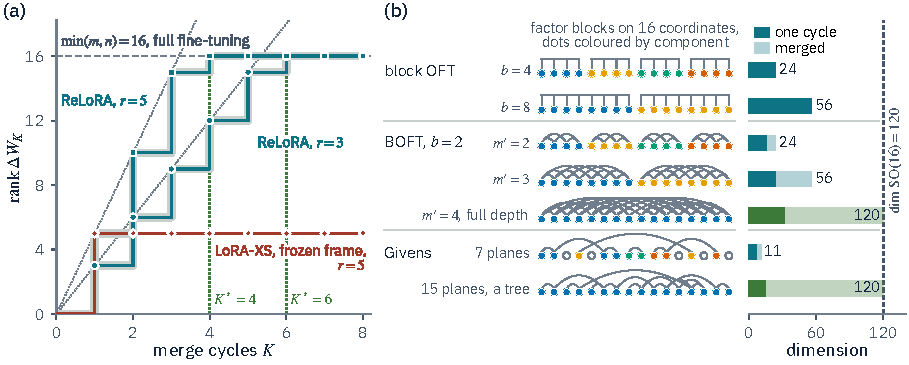
\includegraphics[width=\linewidth]{figures/rebase}
\caption{\textbf{Rebasing reach} (\thmref{Theorem}{V.3}). (a)~The rank staircase for $m\times n=24\times16$: the rank of $\Delta W_K=\sum_{k\le K}B_kA_k$ after $K$ merge-and-restart cycles of ReLoRA, each adding a fresh random rank-$r$ product, for $r=3$ (circles) and $r=5$ (squares). The measured ranks (teal) lie on the bound $\min(Kr,m,n)$ (thick grey; dotted, the line $Kr$) at every $K$, so ReLoRA reaches full rank exactly at $K^*=\lceil16/r\rceil$ cycles, and not before (corollary~1, \thmref{Theorem}{V.3}(a)). LoRA-XS with its frames frozen at the injective base $W_0$ (red, $r=5$) stays at rank $5$: an idempotent method gains nothing from rebasing (corollary~2). (b)~Seven families of block-orthogonal factors on $n=16$ coordinates: block OFT on a fixed partition with blocks of size $b=4$ and $b=8$, BOFT with $b=2$ and $m'=2,3,4$ butterfly factors, and Givens rotations in $7$ planes and in $15$ planes forming a spanning tree. Arcs are two-element blocks and brackets larger blocks; dots are coloured by the connected component of the hypergraph the blocks generate, and hollow dots are isolated coordinates. The light bars give the dimension $\sum_C\binom{\lvert C\rvert}{2}$ of the generated Lie algebra (\thmref{Theorem}{V.3}(c)), and the dark bars the dimension reached in one cycle, against $\dim\mathrm{SO}(16)=120$ (dashed), with green bars for the families that reach it. Only a connected hypergraph reaches $120$; for BOFT that takes the full depth $m'=4$ (corollary~4). The bar values are in \S\ref{app:repro-figures}.}\label{fig:rebase}
\end{figure}

\begin{theorem}{V.3}{rebasing closure}
(a) \emph{Additive methods with a fixed shape $C\ni0$}, with frames, masks and compression operators frozen at
$\theta_0$ across cycles. Then $R_K=\theta_0+C^{+K}$, the $K$-fold Minkowski sum, and
$R_\infty=\theta_0+\operatorname{Mon}(C)$, the additive monoid generated by $C$ (\bgref{D.10}). If $C$ is closed under
real scalings, $R_\infty=\theta_0+\spanop C$.

(b) \emph{Action methods}, where one cycle applies an element of a set $S$ with $1\in S\subseteq G$; for scaling
methods, $S\subseteq\operatorname{End}(\Theta)$ is a subset containing the identity. Then $R_K=S^K\theta_0$, and
$R_\infty$ is the orbit of the monoid generated by $S$. Suppose $S$ lies in the subgroup generated by connected Lie
subgroups $H_1,\dots,H_p$ (\bgref{D.8}) and contains a neighbourhood of $1$ in each. Then the monoid generated by $S$ is
the connected Lie subgroup $H$ with $\operatorname{Lie}(H)=\operatorname{Lie}\langle\mathfrak h_1,\dots,\mathfrak
h_p\rangle$.

(c) \emph{Block-orthogonal factors.} Let the factors have coordinate blocks $I_j\subseteq\{1,\dots,n\}$ (block OFT,
BOFT factors, Givens planes). Then
\[\operatorname{Lie}\langle\so(I_j)\rangle_j=\bigoplus_C\so(C),\]
summed over the connected components $C$ of the hypergraph $(\{1,\dots,n\},\{I_j\})$.

\emph{Corollaries.}
\begin{enumerate}[label=\arabic*.,leftmargin=1.6em]
  \item \textbf{ReLoRA} \citep{lialin2023relora}. $R_K=W_0+\MM_{\le\min(Kr,m,n)}$. It reaches full fine-tuning iff
  $K\ge\lceil\min(m,n)/r\rceil$.
  \item \textbf{Idempotent methods} gain nothing from rebasing. These are the methods whose shape is exactly a
  subspace, subgroup or submonoid independent of the base, with frames, masks and compression operators frozen across
  cycles. Examples are LoRA-FA with a fixed $A$ \citep{zhang2023lora}, LoRA-XS with frozen frames
  \citep{baazy2024lora}, MoRA with fixed operators \citep{jiang2024mora}, FourierFT with fixed indices
  \citep{gao2024parameter}, WaveFT \citep{bilican2025exploring}, C3A \citep{chen2024parameter}, MiSS
  \citep{kang2024miss} (default balance mode; bat mode is base-dependent but still idempotent, since its blockwise maps
  $W\mapsto(W+I)(I+M)-I$ form a monoid), SHiRA \citep{bhardwaj2024sparse}, BitFit \citep{benzaken2021bitfit}, FISH
  with a fixed mask \citep{sung2021training}, LN-tuning \citep{zhao2023tuning}, (IA)$^3$ \citep{liu2022few}, SSF
  \citep{lian2022scaling} and RoAd \citep{liao20243}. Block OFT with a fixed partition and an exact Cayley map gains
  only the measure-zero set of block rotations with an eigenvalue $-1$, so $R_\infty=W_0\cdot\prod\SO(b)=\overline{R_1}$.
  Constrained OFT (COFT, an $\varepsilon$-ball) with an exact Cayley map gains up to $\prod\SO(b)$; HF's
  \texttt{coft=True} keeps the Cayley--Neumann map by default and so falls under corollary~4. Methods that recompute
  frames or masks from the merged weight (an SVD-recomputing LoRA-XS, ReMoRA's alternating operators, resampled
  indices) do gain.
  \item \textbf{VeRA} \citep{kopiczko2023vera}. $\mathrm{VeRA}^\infty=\text{LoRA-FA}(A)$ whenever the frozen $B$ has no
  zero entries.
  \item \textbf{OFT family.} Block OFT with an exact Cayley map is stuck in $W_0\cdot\prod\SO(b)$. HF's default
  Cayley--Neumann factor is $R=C(Q)(I-Q^4)$, with $C$ the exact Cayley map (\bgref{D.7}), so $R\T R=(I-Q^4)^2$ and $R$
  is not orthogonal. Its singular values are $\lvert1-\mu_k^4\rvert$, where $\pm i\mu_k$ are the eigenvalues of $Q$.
  In the operating regime $\lVert Q\rVert_{\rm op}\le2^{1/4}$ (every $\mu_k\le2^{1/4}$), the regime the truncated series
  is meant for, every factor is a contraction. Re-merging then decreases $K_{\rm out}$ in the Loewner order and no
  singular value grows, so the drift is monotone shrinkage, and the reachable set lies in $W_0$ times the block
  contraction semigroup. With unconstrained $Q$ the factors include singular ones ($\mu_k=1$), and re-merging
  generates $\prod\big(\GL^+(b)\cup\MM_{\le b-2}\big)$, or $\prod\big(\CO^+(2)\cup\{0\}\big)$ when $b=2$; this clause
  is established at the level of a proof sketch. Iterated BOFT (exact Cayley in HF) with $m'$ butterfly factors of
  block size $b$ reaches
  \[\diag(\R^m)\cdot W_0\cdot P\Big(\prod\SO\big(b\,2^{m'-1}\big)\Big)P\T,\]
  because the factor hypergraph has components of size $b\,2^{m'-1}$. For injective $W_0$ this is
  $\diag(\R^m)\cdot W_0\cdot\SO(n)$ iff $b\,2^{m'-1}=n$, the full-depth butterfly $m'=1+\log_2(n/b)$. HF's default \texttt{boft\_\allowbreak n\_\allowbreak butterfly\_\allowbreak factor=1} is
  block OFT times $\diag(s)$. A \emph{single} full-depth BOFT has dimension at most $m'\tfrac nb\binom b2$, which is
  below $\dim\SO(n)$ when $m'(b-1)<n-1$; its matrices are dense, while the set they form has positive codimension.
  \item \textbf{Re-HRA} (HF \texttt{apply\_GS=False}), with $W_0$ injective and $r$ even. Then
  $R_K=(W_0+\MM_{\le Kr})\cap W_0\cdot\SO(n)$, so \emph{rebasing commutes with the meet} of \thmref{Theorem}{II.7}.
  This multiplicative twin of ReLoRA reaches $W_0\cdot\SO(n)$ in at most $\lceil n/r\rceil$ cycles.
  \item \textbf{GaLore (with a gradient-SVD or a random projector), LISA and MeZO}, under the optimizer hypotheses of
  \thmref{Proposition}{IV.2}, are rebasing schemes of \emph{linear} methods whose shape moves. That is why, as a set
  over the sequences of shapes they can choose, they reach all of $\Theta$, while a fixed linear shape $L$ reaches
  only $\theta_0+L$ (corollary~2). Low rank is the per-period obstruction only for GaLore; LISA and MeZO already make
  full-rank per-matrix updates and gain coverage. Flora proper takes full-space steps with a compressed momentum, so
  it has no per-period low-rank shape.
  \item \textbf{Merging never rescues an exactly orthogonal method from its absolute invariants.} In exact arithmetic,
  every exactly orthogonal input-side rebasing preserves $K_{\rm out}$ and the spectrum, and every output-side one
  preserves $K_{\rm in}$ and the spectrum (\thmref{Corollary}{II.6}).
\end{enumerate}
\end{theorem}

\paragraph{Numerical check} For the butterfly hypergraph at $n=64$, $b=4$, the components have sizes $4,8,16,32,64$
for $m'=1,\dots,5$, so it is connected only at $m'=5$; an independent check with HF's own permutation code gives the
same sizes. The Lie algebra generated by the Cayley--Neumann factors at $b=4$ has dimension $16=\dim\gl(4)$. With skew
entries of size about $0.05$, $K_{\rm out}$ moves by $0.2\%$, $1\%$, $6\%$ and $22\%$ (relative) after $1$, $10$, $50$
and $200$ default-OFT merges, decreasing in the Loewner order at every merge. Random skew $Q$ with
$\lVert Q\rVert_{\rm op}\le2^{1/4}$ never give $\lVert R\rVert_{\rm op}>1$, and at $b=2$ the generator
$Q=\left(\begin{smallmatrix}0&-1\\1&0\end{smallmatrix}\right)$ gives $R=0$ (Appendix~\ref{app:repro}).

\paragraph{Credit} Merge-and-restart training is ReLoRA \citep{lialin2023relora}. The orthogonal methods are OFT
\citep{qiu2023controlling}, with its constrained variant COFT, BOFT \citep{liu2023parameter}, whose butterflies come from
\citet{dao2019learning}, and HRA \citep{yuan2024bridging}, whose Householder products go back to
\citet{mhammedi2016efficient}. Cayley parametrisations of orthogonal layers are studied in
\citet{lezcanocasado2019cheap}. The group theory is classical. It uses Yamabe's theorem on arcwise connected subgroups
\citep{xyamabe1950arcwise} (\bgref{D.9}) and Scherk's sharp form of the Cartan--Dieudonné theorem
\citep{xscherk1950decomposition} (\bgref{D.11}). That GaLore \citep{zhao2024galore} is one-sided LoRA re-based every
period is due to \citet{xtorrobahennigen2025duality}, and the random-projection case to Flora \citep{hao2024flora}; see
\thmref{Proposition}{IV.2}. The other moving-shape methods are LISA \citep{pan2024lisa} and MeZO
\citep{malladi2023fine}.

\begin{table}[t]
\centering\footnotesize
\caption{What merge-and-restart reaches (\thmref{Theorem}{V.3} and its corollaries).}\label{tab:base-rebasing}
\begin{tabularx}{\linewidth}{@{}>{\raggedright\arraybackslash}p{0.25\linewidth}>{\raggedright\arraybackslash}p{0.19\linewidth}>{\raggedright\arraybackslash}X>{\raggedright\arraybackslash}p{0.2\linewidth}@{}}
\toprule
\headrow \textbf{Method under rebasing} & \textbf{One cycle} & \textbf{After $K$ cycles, or $R_\infty$} &
\textbf{Gain from restarting} \\
\midrule
ReLoRA \citep{lialin2023relora} & $W_0+\Mr$ & $W_0+\MM_{\le\min(Kr,m,n)}$ & yes; full FT at
$K\ge\lceil\min(m,n)/r\rceil$ \\
\addlinespace
LoRA-FA (fixed $A$), LoRA-XS (frozen frames), BitFit, (IA)$^3$, SSF, fixed masks & a subspace or submonoid & the same
set & none (idempotent) \\
\addlinespace
VeRA \citep{kopiczko2023vera} ($B$ without zero entries) & $W_0+\Lambda_bB\Lambda_dA$ & $\text{LoRA-FA}(A)$ & yes, up to
LoRA-FA \\
\addlinespace
block OFT \citep{qiu2023controlling}, exact Cayley, fixed partition & $W_0\cdot\prod\mathrm{Cay}(b)$ &
$W_0\cdot\prod\SO(b)=\overline{R_1}$ & measure zero \\
\addlinespace
COFT, exact Cayley & an $\varepsilon$-ball in each block & up to $W_0\cdot\prod\SO(b)$ & within the blocks \\
\addlinespace
block OFT, HF Cayley--Neumann default & not orthogonal & a contraction monoid for small $Q$ & drifts; $K_{\rm out}$
shrinks \\
\addlinespace
BOFT \citep{liu2023parameter}, $m'$ butterfly factors, exact Cayley & products of butterfly factors &
$\diag\cdot W_0\cdot P\big(\prod\SO(b\,2^{m'-1})\big)P\T$ & $\SO(n)$ iff $b\,2^{m'-1}=n$ \\
\addlinespace
re-HRA \citep{yuan2024bridging} ($W_0$ injective, $r$ even) & $(W_0+\Mr)\cap W_0\cdot\SO(n)$ &
$(W_0+\MM_{\le Kr})\cap W_0\cdot\SO(n)$ & yes; $W_0\cdot\SO(n)$ within $\lceil n/r\rceil$ \\
\addlinespace
GaLore, LISA, MeZO & a linear shape that moves & all of $\Theta$, as a set & yes, because the shape moves \\
\bottomrule
\end{tabularx}
\end{table}

\begin{explains}
ReLoRA is \thmref{Observation}{I.7} unrolled in time, since a sum of $K$ rank-$r$ LoRAs is one LoRA of rank $Kr$, so it
walks the group its cone generates. A fixed additive shape gains from restarts only when it is not closed under
addition, as LoRA's cone and VeRA's shape are not. Exact-Cayley block OFT can never escape its $n/b$ partial-Gram
invariants however often it is re-merged. Butterfly permutations exist precisely to connect the block hypergraph, and
they connect it fully only at full depth.
\end{explains}

\begin{remark*}{2026: POET-X}
POET-X \citep{qiu2026poet}, a pretraining method whose $W_0$ is a random initialisation, changes the partition between
cycles, on both sides of the weight. Each round trains a block-diagonal factor conjugated by a random permutation on
each side, merges both into the weight and redraws the permutations. With exact Cayley blocks every merged weight lies
in $\SO(m)\,W_0\,\SO(n)$, so it keeps the singular values of $W_0$ (\thmref{Theorem}{II.5}), and by
\thmref{Theorem}{V.3}(b) and (c) blocks that together connect all coordinates of a side generate all of $\SO$ on that
side. Its blocks are in fact $(I+Q)(I+Q+Q^2+Q^3)$, the Cayley--Neumann factor of corollary~4, so while every
$\mu_k\le2^{1/4}$ no merge raises a singular value, and the spectrum can only drift down.
\end{remark*}

\begin{example*}{one projection of a 7B model}
Take a $4096\times4096$ projection. ReLoRA with $r=16$ reaches full fine-tuning after $256$ cycles and not before. For
injective $W_0$, re-HRA with $r=8$ reaches $W_0\cdot\SO(4096)$ within $512$ cycles. BOFT with $b=4$ needs $m'=11$
butterfly factors before re-merging reaches that orbit up to output scaling; at HF's default of one factor it stays in
$W_0\cdot\prod\SO(4)$ up to the scale. A single 11-factor BOFT has dimension at most $11\cdot1024\cdot6=67{,}584$,
against $\dim\SO(4096)=8{,}386{,}560$.
\end{example*}

\paragraph{Prediction} With an exact Cayley map and a fixed partition, re-merging adds nothing to block OFT's reach
beyond closure, so re-merged exact-Cayley block OFT and COFT on a fixed partition never leave $W_0\cdot\prod\SO(b)$.
Enlarging the reach needs a connected block hypergraph (partitions that change between cycles, or full-depth
butterflies) or a COFT ball. LoRA-type cones gain from rebasing with a fixed shape, while linear additive shapes do not
(corollary~2). These are statements about reach; whether extra reach improves a trained model is the experiment
(\thmref{Prediction}{X.6}).

\subsubsection{Combining: rules that must ignore the gauge}\label{sec:base-combine}

A LoRA module ships as factors $(B,A)$, the model sees only $BA$, and $(Bg^{-1},gA)$ gives the same product for every
$g\in\GL_r$. A combination rule should return the same model for every choice of factors, or two people with the same
adapters can merge them into different models. Task arithmetic adds the products and passes. LoraHub adds the $B$'s,
adds the $A$'s and multiplies, and fails, because its cross terms $B_iA_l$ see a rescaling $(cB,A/c)$ of one module.
The merge panel of Figure~\ref{fig:gauge} shows the LoraHub merge moving under that rescaling while task arithmetic
stays fixed.

\begin{proposition}{V.4}{combination rules: gauge and naturality}
(a) A rule $\Phi\big((B_i,A_i)_i\big)$ for combining LoRA factors descends to a function of the adapters $(B_iA_i)_i$
iff it is constant on the fibres of $(B_i,A_i)\mapsto(B_iA_i)$. On the full-rank locus this is equivalent to
$\prod_i\GL_r$-invariance. It is also equivalent for $\Phi$ continuous on the whole factor space; this clause rests on
the unique closed orbit in each fibre, which lies in the closure of every orbit of the fibre (\bgref{D.31}).
\begin{itemize}
  \item Task arithmetic $\sum_iw_is_iB_iA_i$, with $s_i$ HF's \texttt{scaling} ($\alpha_i/r_i$, or $\alpha_i/\sqrt{r_i}$
  under rsLoRA), is invariant and lands in $\mathrm{LoRA}_{\sum_ir_i}$. It is HF's \texttt{cat} with merged scale $1$
  (\thmref{Observation}{I.7}).
  \item LoraHub's factor-wise rule $\big(\sum_iw_iB_i\big)\big(\sum_jw_jA_j\big)$ is not invariant. Replacing
  $(B_2,A_2)$ by $(cB_2,A_2/c)$ changes it by
  \[\sum_{l\ne2}w_lw_2\big[(c-1)B_2A_l+(c^{-1}-1)B_lA_2\big].\]
  HF's \texttt{add\_\allowbreak weighted\_\allowbreak adapter(..., combination\_\allowbreak type="linear")} is a
  factor-wise rule of the same type. It weights $A_i$ by $\operatorname{sign}(w_i)\sqrt{\lvert w_is_i\rvert}$ and $B_i$
  by $\sqrt{\lvert w_is_i\rvert}$ and sums the factors separately, so it has cross terms. On adapters that share a
  frozen $A$ it is still not exact up to a global factor, since the relative weights become
  $\sqrt{\lvert w_is_i\rvert}$. HF's non-SVD \texttt{ties}, \texttt{dare\_*} and \texttt{magnitude\_prune} variants
  also act on factors; the \texttt{*\_svd} variants act on full updates.
  \item Poly and MHR are different. Their skill inventories are trained jointly through the product-of-sums map, which
  is invariant under the diagonal $\GL_r$, one common $g$ for every skill. Numerically, for fixed generic routing with
  fewer skills than tasks and full-rank factors, this is the whole continuous fibre. With at least as many skills as
  tasks, or once the routing is counted as a parameter, there are further symmetries (skill permutations, and
  re-mixings $\alpha\mapsto\alpha M$ with $M\mathbf 1=\mathbf 1$). Their cross terms are a design choice of a jointly
  trained parametrisation, and raise no question of well-definedness.
\end{itemize}

(b) \emph{Well-definedness versus exactness.} A joint gauge fixing makes a factor-wise rule well defined. For
rank-preserving product-of-sums rules, exactness (agreement with task arithmetic for all weights $w$) needs degree one
in $w$, which for injective factors forces a shared factor; \texttt{cat}, which concatenates and raises the rank, is
exact without one. A frozen shared factor (FFA-LoRA; LoRA-FA) gives $\big(\sum_iw_iB_i\big)A=\sum_iw_iB_iA$ exactly.
LoraHub with a shared $A$ still returns $\big(\sum_jw_j\big)\sum_iw_iB_iA$, exact only up to the global factor
$\sum_jw_j$, since its weights are unnormalised. A per-module SVD canonical form leaves a $(\mathbb Z/2)^r$ of sign
flips per module, plus rotations within repeated singular values, and these change the cross terms. What is needed is
a \emph{joint} frame that produces a shared factor, as KnOTS's joint re-factorisation of the concatenated updates
through a shared $U\Sigma$ does. Federated LoRA shows the difference. FedAvg-LoRA clients start each round from the
same broadcast $(B,A)$, so their failure,
\[\tfrac12(B_1+B_2)\cdot\tfrac12(A_1+A_2)\ne\tfrac12(B_1A_1+B_2A_2),\]
is bilinearity, and it persists in a fully fixed gauge.

(c) \emph{Naturality.} On updates with $N$ coordinates, write $T_N$, $B_N$ and $\mathrm{Mon}_N$ for the invertible
diagonal, signed permutation and monomial matrices. Task arithmetic is $\GL(\Theta)$-equivariant on updates. DARE is
coordinatewise and magnitude-free, $D(m\odot\tau)=m\odot(D\tau)$ for every invertible diagonal $D$ and the same mask
$m$. So DARE is exactly equivariant under the torus $T_N$, sign flips included, for each mask, and under permutations in
distribution; its distributional group is exactly $\mathrm{Mon}_N$. TIES with global trimming (top-$k$ magnitude, sign
election by total mass as in the TIES paper and HF's default \texttt{"total"}, disjoint mean) is equivariant under
$\R^\times\cdot B_N$, homotheties times signed permutations, generically (off magnitude ties at the threshold). With
HF's \texttt{majority\_\allowbreak sign\_\allowbreak method="frequency"}, count ties are broken to $+1$ and the group
drops to $\R_{>0}\cdot S_N$. Per-tensor trimming changes the group to $\prod_b\big(\R^\times\cdot B_{N_b}\big)$,
extended by permutations of equal-size blocks. DARE followed by full TIES (with trimming) is
$\R^\times\cdot B_N$-equivariant in distribution; HF's and MergeKit's \texttt{dare\_ties} has no magnitude trim, so
with \texttt{"total"} election it is exactly $T_N$-equivariant per mask, and its group contains $\mathrm{Mon}_N$. None
of the sparsifying rules (DARE, TIES, DARE-TIES) is $\Ort(N)$-equivariant. Applied to factors and summed across adapters
(HF's non-SVD variants), all of them are gauge-dependent, and under independent per-adapter gauges even DARE fails,
through the cross terms of (a). DARE's masking commutes with $T_r$ exactly for each mask and with $\mathrm{Mon}_r$ in
distribution, so a single masked adapter, or a factor-wise sum under one gauge shared by all adapters, is
$T_r$-invariant per mask and $\mathrm{Mon}_r$-invariant in distribution.
\end{proposition}

\paragraph{Numerical check} DARE with a random non-unit diagonal $D$ is equivariant to $2\times10^{-15}$ per mask.
TIES is homogeneous to $9\times10^{-16}$ and fails by $5.6$ under a generic positive diagonal. The general LoraHub
change formula matches with three modules to $2\times10^{-15}$. On the factors of two adapters, a diagonal gauge on one
of them moves factor-wise DARE by an amount of order one, while the same gauge shared by all adapters leaves it fixed to
$10^{-15}$. For Poly with $3$ skills, $r=2$ and $6\times6$ weights, the fibre has dimension $32$ with $2$ tasks and
$4=\dim\GL_2$ with $4$ tasks (Appendix~\ref{app:repro}).

\paragraph{HF options} With HF's \texttt{majority\_\allowbreak sign\_\allowbreak method="frequency"}, sign counts are
integers, so ties are common, and they are broken towards $+1$. Sign flips and negative homotheties therefore fail for
\texttt{ties} and \texttt{dare\_ties} alike.

\paragraph{Credit} The rules studied here are task arithmetic \citep{ilharco2022editing}, LoraHub
\citep{huang2023lorahub}, TIES \citep{yadav2023ties}, DARE \citep{yu2023language} and KnOTS \citep{stoica2024model},
whose joint SVD is the shared frame of (b); \texttt{dare\_ties} is as implemented in HF PEFT
\citep{xmangrulkar2022peft} and MergeKit \citep{xgoddard2024mergekit}. Jointly trained skill inventories are Poly
\citep{ponti2022combining} and MHR \citep{caccia2022multi}. Federated averaging of LoRA factors is used in FedIT
\citep{zhang2023building}, and the frozen shared factor that removes its bilinearity is FFA-LoRA
\citep{sun2024improving}. That functions of LoRA weights should respect their $\GL_r$ symmetry is the starting point of
the $\GL$-equivariant networks of \citet{putterman2024learning}; for full models, hidden-unit permutations play that
role in Git Re-Basin \citep{ainsworth2022git}. The unique closed orbit in each fibre is classical invariant theory.
\citet{xkempf1979length} characterise closed orbits by norm-minimising points (\bgref{D.30}), here the balanced
factorisations of \thmref{Proposition}{III.7}, and \citet{xrichardson1990minimum} treat real groups. For optimizers,
the same question leads to \citet{zhang2024riemannian} and \citet{yen2024lora}; see \thmref{Theorem}{III.12}.

\begin{explains}
Post-hoc factor merging of independently trained modules, as in LoraHub and HF's \texttt{linear}, is not a function of
the adapters. It depends on how each module happened to be factorised, which nobody controls after training. Federated
LoRA fails through bilinearity instead, and FFA-LoRA's frozen shared factor repairs it. KnOTS's joint
re-factorisation produces a shared factor. \textbf{Design rule: combine LoRAs on products, or only after a joint
re-factorisation that produces a shared factor.}
\end{explains}

\paragraph{Prediction} LoraHub behaves like update arithmetic, up to the factor $\sum_jw_j$, when its modules share
the $A$-seed and $A$ stays close to its initialisation. That regime is empirical and favoured by a large ratio
$\eta_B/\eta_A$, as in LoRA+ \citep{hayou2024lora}. LoraHub degrades when the modules come from independent seeds
(\thmref{Prediction}{X.9}).

\subsubsection{What base change leaves for the network}\label{sec:base-next}

Every move here stayed inside weight space, where merging into the base is the canonical arrow to the terminal object
of \thmref{Observation}{I.4} and always exists. Adapters, prefixes and ReFT change the network itself, and for them
merging is a lifting problem whose obstructions the activation function decides. That is Exposé~\ref{sec:merge}.
